\section{Build \& Run}
The generation and execution of each part of the system and
the whole system itself comprised two steps:

\begin{itemize}
   \item \texttt{build} - this step is necessary to download and create all the docker
   images and generate the configuration files both for the simulator and the
   template configurations for docker
   (e.g., define in which mode you want the system to run and
   which components need to be instantiated).
	Basically, this step
   corresponds to the installation of the product.
   \item \texttt{run} - this step requires docker-swarm
	or only docker-compose depending on the configurations chosen for the build
	\footnote{for simplicity we provide only the complete system configuration and not the
	only-single-component deployment. However, during the development of the project
	the system has been used with the latter configurations.
	It would be quite easy to provide all the possible configurations}.
	If you have chosen to configure the whole system, then docker swarm deploys the system
   as a composition of stacks: each stack is a set of services which represent
   a city. However, the AMQP broker and the Viewer are wrapped in a separated
   stack which is unique within the system (i.e., does not depend upon the
   number of cities). Note that the size of each city and the number of deployed
   cities remarkably affect the time required to complete this process.
	It will generally last as long as the number of cities chosen will be greater.
\end{itemize}

A logical view which exemplifies the deployed system is depicted in Figure
\ref{fig:deploy-sys}.

\begin{figure}[H]
\centering
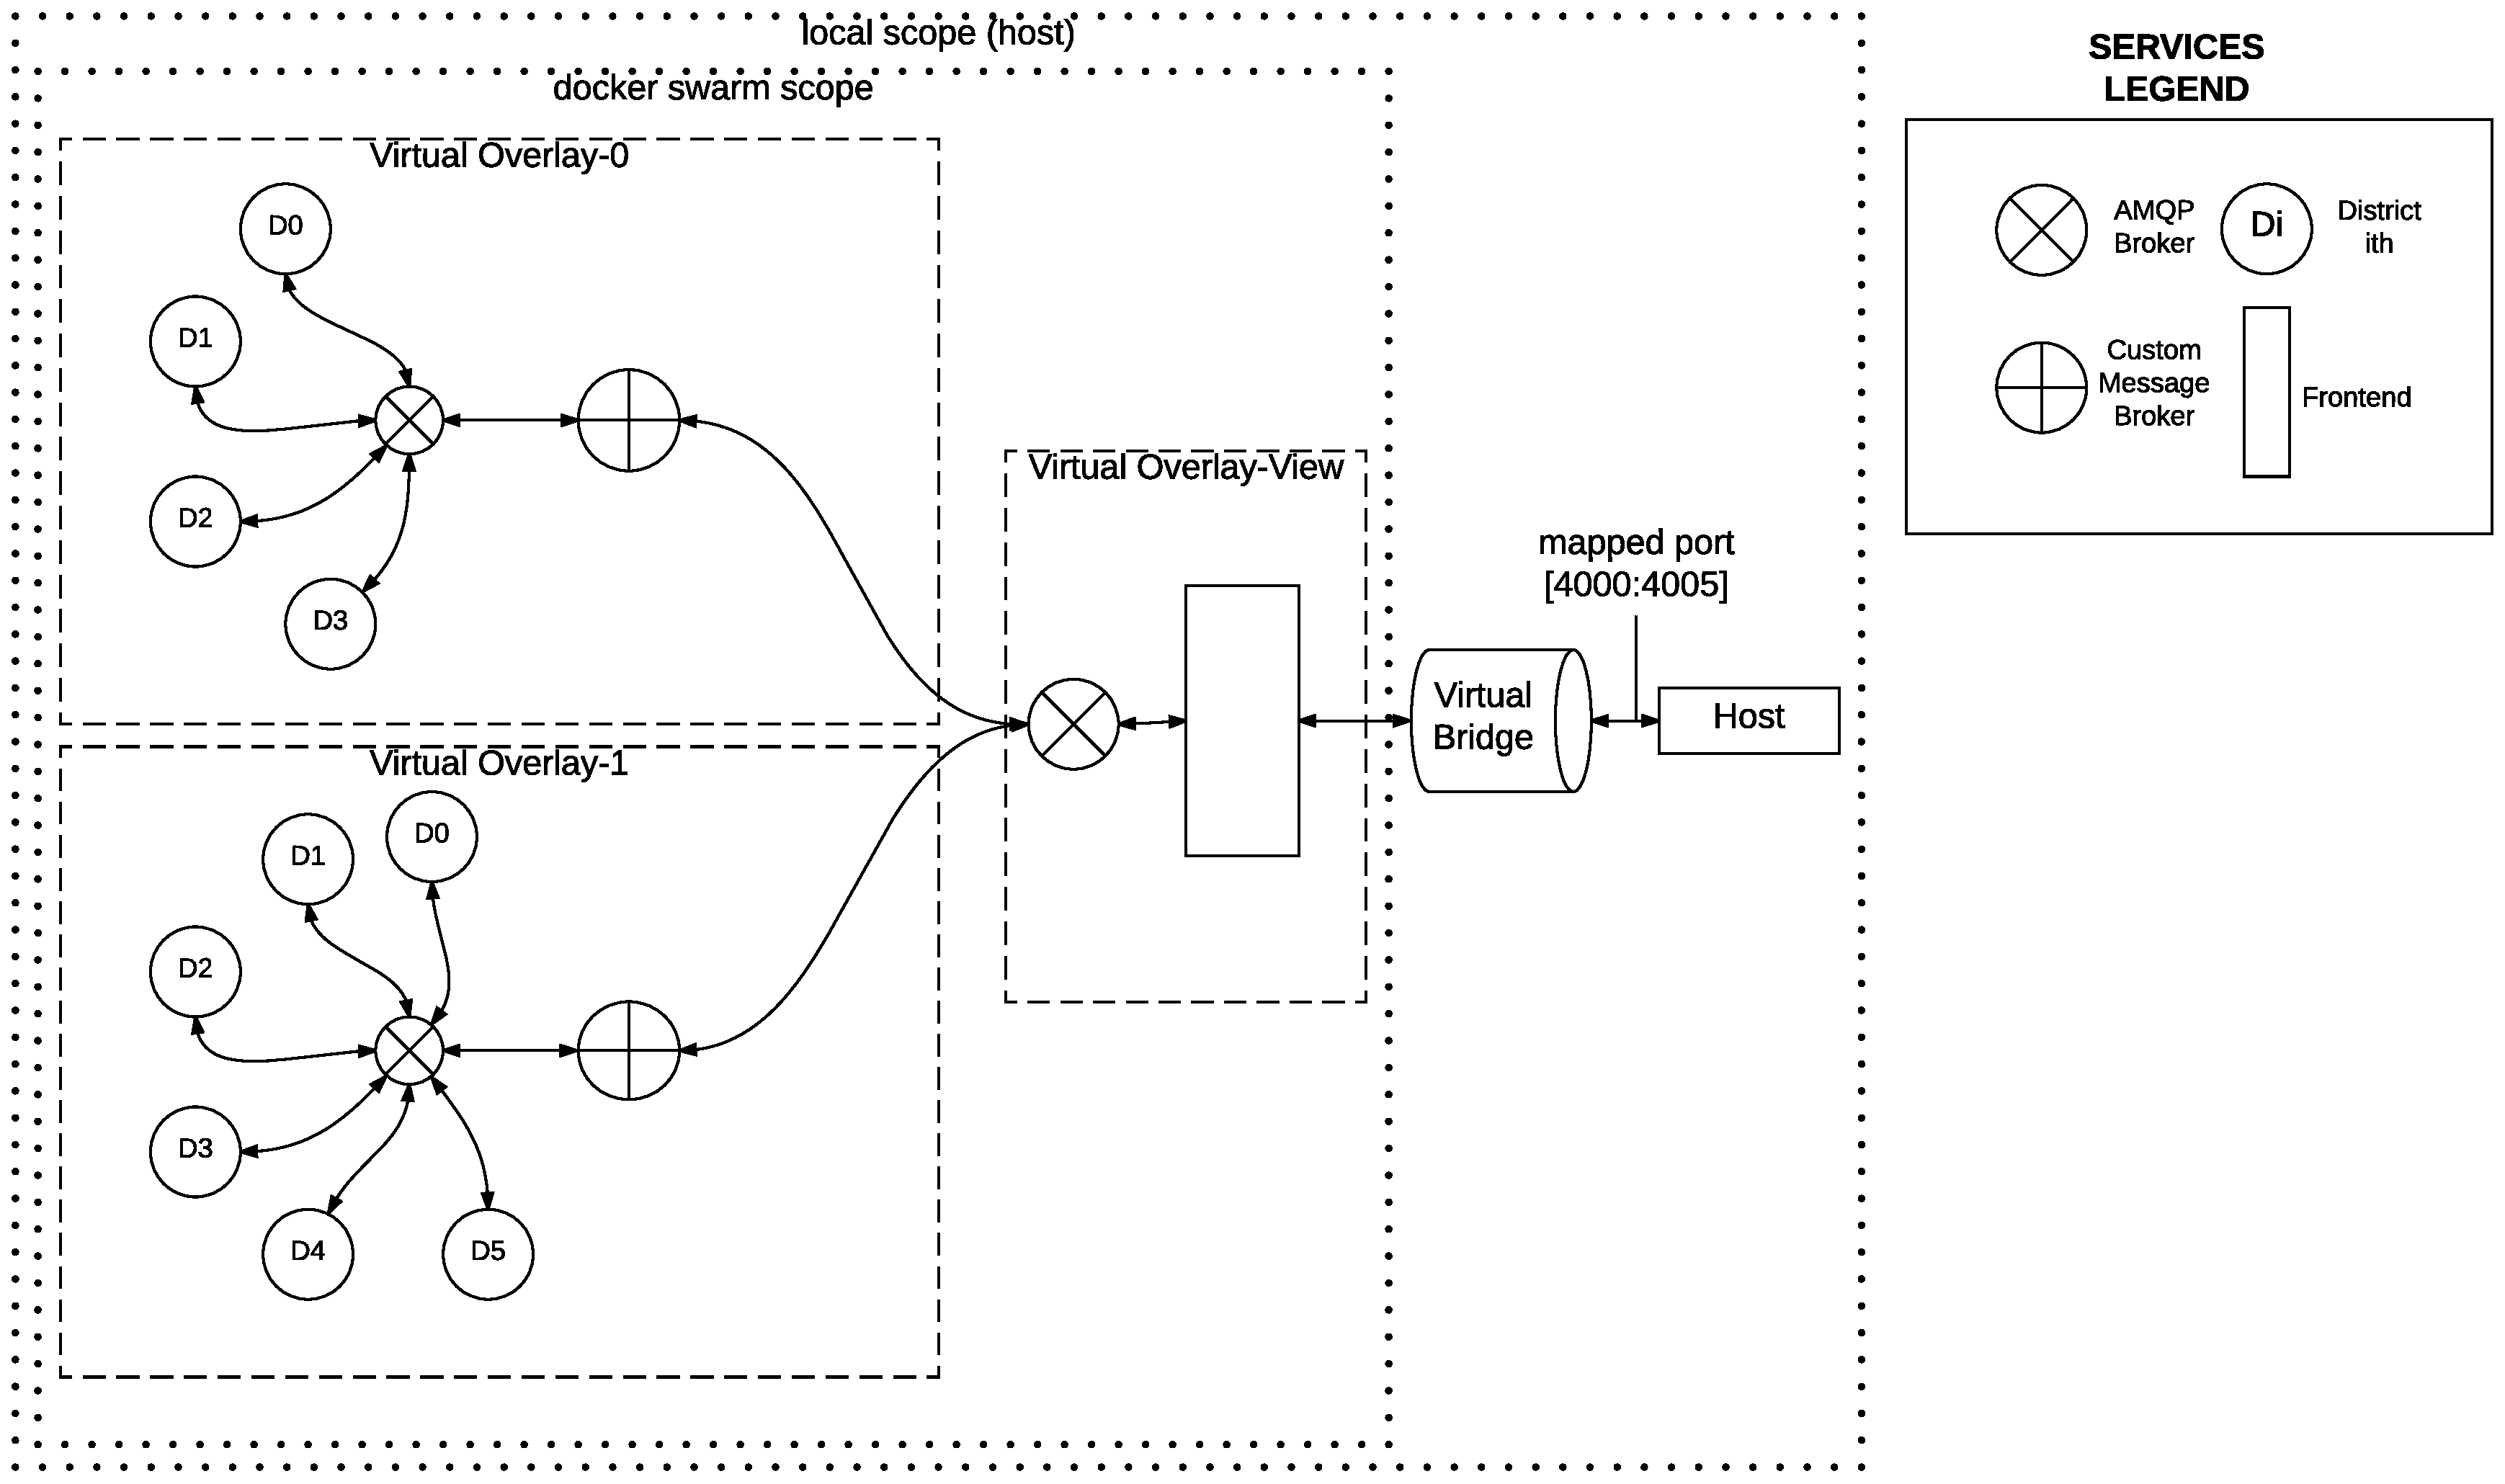
\includegraphics[scale=0.5,keepaspectratio]{images/user-man/eps/deploy.eps}
\caption{Example of a deployed ACTS system}
\label{fig:deploy-sys}
\end{figure}
